\chapter{Vliv odchylek v parametrech na přesnost modelu}

Pro vytvoření modelu spotřeby elektrické energie průmyslového robota je potřeba identifikovat mnoho neznámých parametrů. V případě robota KUKA KR5 Arc se jedná o celkem 54 neznámých parametrů. Ne všechny parametry ale ovlivňují dynamiku robota a s ní spojenou spotřebu elektrické energie stejně. Některé parametry mají mnohem větší vliv než jiné. Pro vytvoření co nejpřesnějšího modelu je proto vhodné tyto parametry identifikovat co nejpřesněji. 

V této sekci je provedena analýza vlivu odchylek v jednotlivých identifikovaných parametrech na přesnost modelu. Dynamický model robota je velmi nelineární. Proto není pro analýzu odchylek parametrů možné použít žádnou z lineárních metod, jako je například určení přenosu ze změny parametru na výstupní výkon nebo simulace systému s jednoduchým zvětšením/zmenšením parametrů. 

Z tohoto důvodu je analýza vlivu odchylek v hodnotách parametrů na přesnost energetického modelu robotu provedena použitím metody Monte Carlo. 

\section{Metoda Monte Carlo}

Metody Monte Carlo jsou založeny na vykonání mnoha opakovaných experimentů nebo simulací s náhodně generovanými vstupními parametry za účelem získání numerických výsledků \cite{monte_carlo_ref}. Obdrženou sadu výsledků je poté možné analyzovat analytickými nebo stochastickými metodami. Základní myšlenkou metod Monte Carlo je použití nahodilosti k řešení problémů, které mohou být v principu deterministické.

Tyto metody jsou používány k řešení problémů, u kterých je obtížné nebo dokonce nemožné požít některou z analytických metod. Nejčastěji jsou tyto metody používány pro simulace systémů s mnoha stupni volnosti (kapaliny, systémy s rozprostřenými parametry, propojené systémy), výpočet vícerozměrných určitých integrálů, vyhodnocování rizik v ekonomii a mnoho dalších. 

Analýza vlivu odchylek v identifikovaných parametrech pomocí metody Monte Carlo byla provedena tak, že ke každému z identifikovaných parametrů $R_i$ byla náhodně přičtena hodnota z rozsahu $p \in [-0.2R_i,0.2R_i]$, se kterou byla provedena simulace a vypočítaná střední odchylka mezi simulací a změřenými průběhy. Pro každý parametr bylo takto provedeno 150 simulací, pokaždé s náhodně vygenerovanou hodnotou. Ostatní hodnoty parametrů zůstaly nezměněné. Rozsah přičítaných hodnot $p \in [-0.2R_i,0.2R_i]$ byl zvolen v okolí nominální hodnoty parametru, aby se pohyboval pouze v okolí lokálního minima.

Po vykonání simulací pro všechny parametry bylo vyhodnoceno, při jakých odchylkách parametrů byl největší rozdíl mezi simulovaným a změřeným průběhem. 

\section{Vyhodnocení}

Vyhodnocené maximální relativní odchylky mezi simulacemi a změřenými průběhy jsou uvedeny v tabulce \ref{tab_odch_parametru}. Hodnoty v tabulce jsou vztaženy ke střední odchylce mezi výkonem vypočítaným pomocí identifikovaného modelu a určeným pomocí měření proudů (viz sekce \ref{dosaz_presnost_sec}). Hodnoty udávají, o kolik se zvýší odchylka ve wattech mezi modelem a měřením vůči původnímu identifikovanému modelu.

\begin{table}[htbp]
  \centering
  \caption{Tabulka maximálních dosažených odchylek vzhledem k odchylkám v parametrech}
    \begin{tabular}{c|cccccccccc}
    \multicolumn{1}{c|}{Osa} & \multicolumn{1}{c}{$I_{xx}$} & \multicolumn{1}{c}{$I_{yy}$} & \multicolumn{1}{c}{$I_{zz}$} & \multicolumn{1}{c}{$d_x$} & \multicolumn{1}{c}{$d_y$} & \multicolumn{1}{c}{$d_z$} & \multicolumn{1}{c}{$m$} & \multicolumn{1}{c}{$f_v$} & \multicolumn{1}{c}{$f_c$} \\
    \hline
    1  & 0     & 0     & 0.349 & 0     & 0     & 0     & 0     &  7.080 & 0.271 \\
    2  & 0.018 & 0.022 & 0.145 & 0.392 & 0.461 & 0     & 0.050 &  6.941 & 0.585 \\
    3  & 0.001 & 0.068 & 0.100 & 0.722 & 0.695 & 0.147 & 5.202 &  0.247 & 0.021 \\
    4  & 0.033 & 0.106 & 0.011 & 0.267 & 0.044 & 0.044 & 6.269 &  0.160 & 0.005 \\
    5  & 0.003 & 0.004 & 0.046 & 0.381 & 0.002 & 0.024 & 0.876 &  0.004 & 0.001 \\
    6  & 0.007 & 0.046 & 0.001 & 0     & 0     & 0.045 & 0.246 &  0     & 0     \\
    \end{tabular}%
  \label{tab_odch_parametru}%
\end{table}%

Z hodnot v tabulce je možné vypozorovat, že největší vliv na přesnost modelu mají koeficienty viskózního tření ($f_v$) osy 1 a 2 a hmotnosti ramen ($m$) os 3 a 4. Na obrázcích \ref{vliv_odch_1} až \ref{vliv_odch_4} jsou znázorněny vlivy jednotlivých odchylek těchto parametrů na celkovou odchylku modelu vůči měření. Na svislé ose je relativní odchylka, o kterou se zvýší střední odchylka modelu vůči měření v závislosti na změně parametru. Na vodorovné ose je pak odchylka v identifikovaném parametru. 

\begin{figure}[h]
    \centering
    \begin{subfigure}[b]{1\textwidth}
        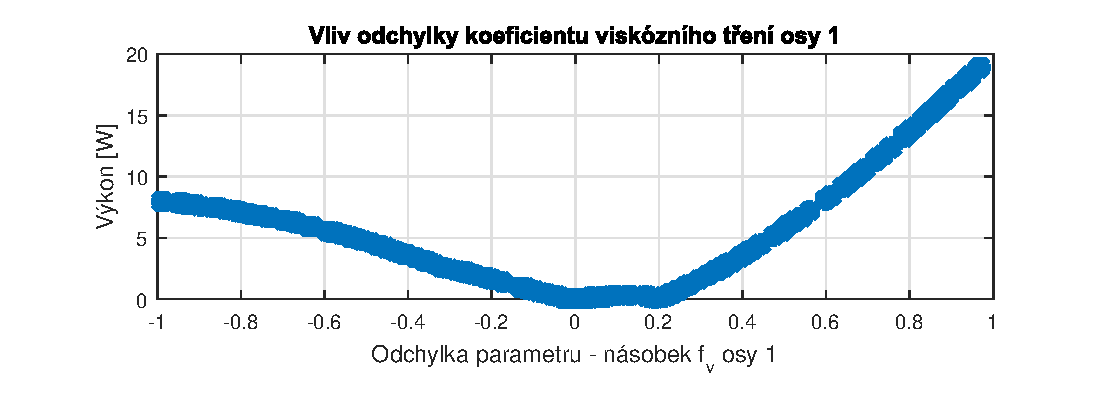
\includegraphics[width=\textwidth]{vliv_odch_osa1_fv}
        \caption{Koeficient viskózního tření osy 1}
        \label{vliv_odch_1}
    \end{subfigure}
    \begin{subfigure}[b]{1\textwidth}
        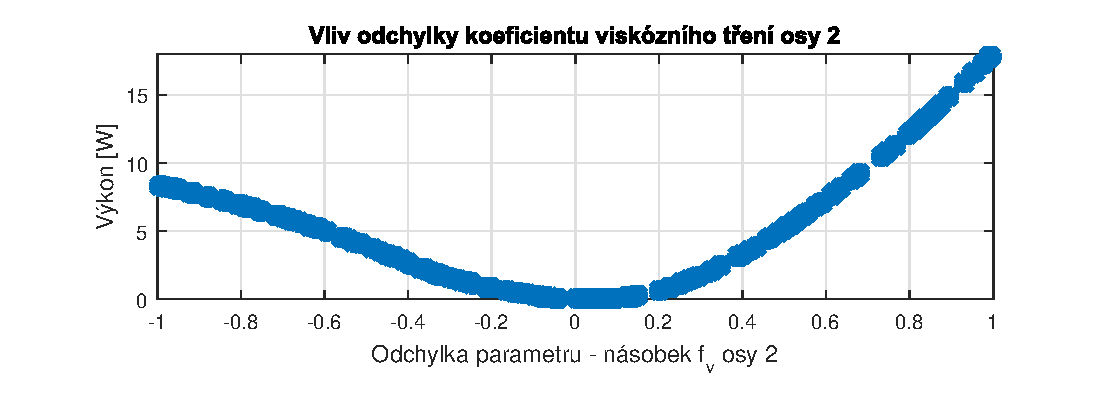
\includegraphics[width=\textwidth]{vliv_odch_osa2_fv}
        \caption{Koeficient viskózního tření osy 2}
        \label{vliv_odch_2}
    \end{subfigure}
    \begin{subfigure}[b]{1\textwidth}
        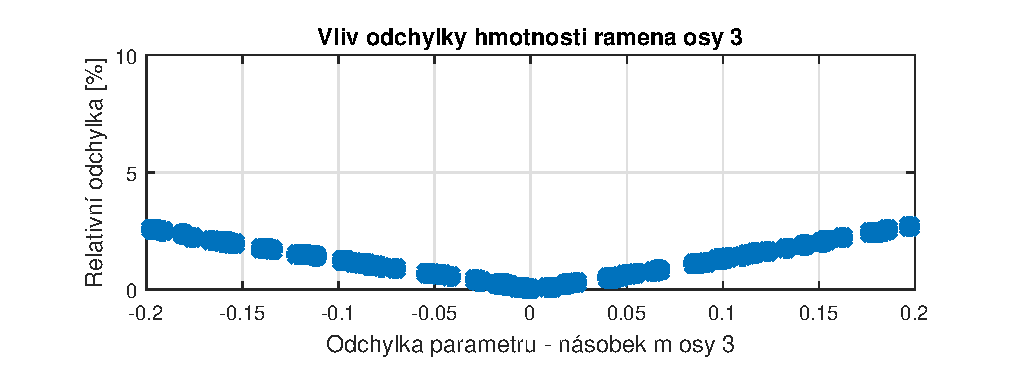
\includegraphics[width=\textwidth]{vliv_odch_osa3_m}
        \caption{Hmotnost osy 3}
        \label{vliv_odch_3}
    \end{subfigure}
    \begin{subfigure}[b]{1\textwidth}
        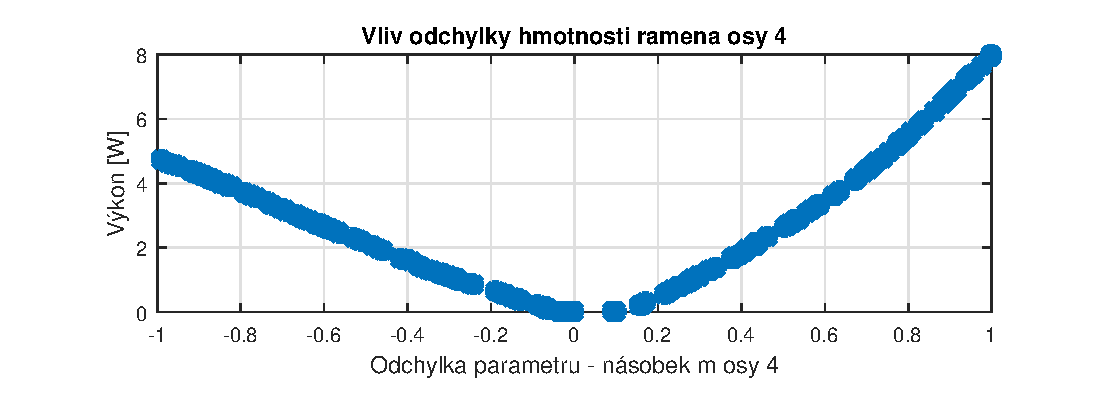
\includegraphics[width=\textwidth]{vliv_odch_osa4_m}
        \caption{Hmotnost osy 4}
        \label{vliv_odch_4}
    \end{subfigure}
    \caption{Vliv odchylek vybraných parametrů na přesnost modelu}
\end{figure} 

\clearpage

Největší vliv na přesnost modelu mají tedy koeficienty tření, hmotnosti a polohy těžišť prvních tří os. Z tohoto důvodu je vhodné si při identifikaci těchto parametrů dát větší pozor a přizpůsobit identifikační excitační trajektorii tak, aby byly identifikovány s co největší přesností.   